\chapter{Optical Detection Technology}
\label{ch:optical}

\begin{figure}[htbp]
    \centering
    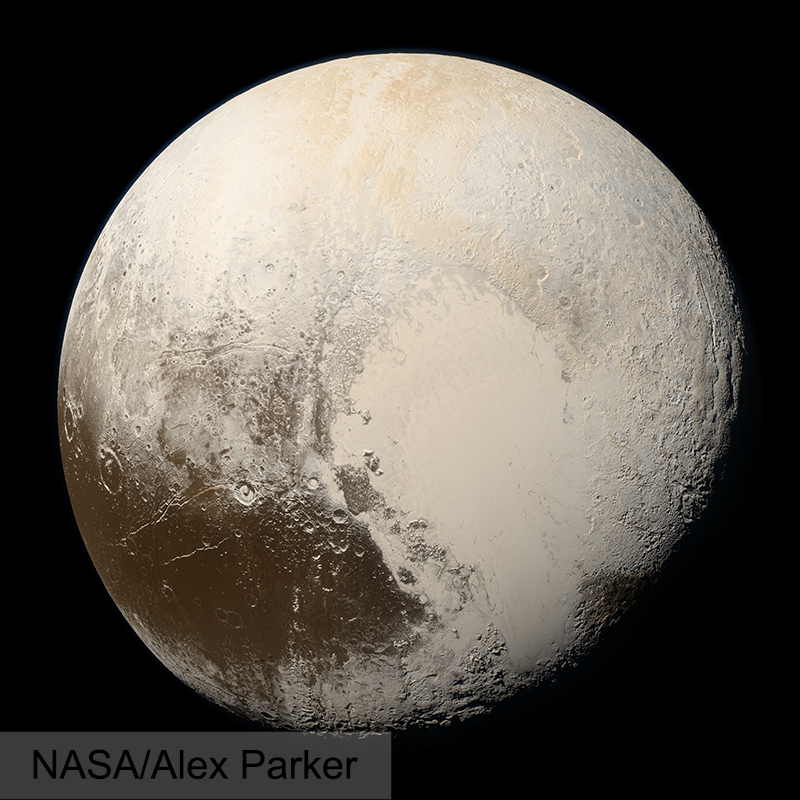
\includegraphics[width=0.5\textwidth]{images/pluto.png}
    \caption{True color image of dwarf planet Pluto taken by the New Horizons space probe in 2015. }
    \label{fig:pluto}
\end{figure}

Optical sensors are some of the most common payloads of modern satellite systems. Ranging from Earth observation, to astronomy, to the cameras used by deep space probes to image their targets, the possibilities of optical sensors to provide detailed and human-interpretable information over large distances have become very mature. Having been used from the start of space exploration (The interested reader is encouraged to read the work of \cite{evolutionofcamera}), optical detection and processing, which will be treated in \autoref{ch:imageprocessing}, have benefited greatly from the advances in semiconductor manufacturing and processing capabilities of modern space systems. From the Vidicon cathode ray tubes in the Voyager probes, spacecraft optical detectors have advanced greatly into modern day charge-coupled devices (CCD) and complementary metal-oxide-substrate (CMOS) detectors.\\

In this chapter, firstly the hardware and software used for optical detection will be discussed in \autoref{sec:opticalhardware}. Then, a fundamental and mathematical discussion of optics and detection hardware will be given in \autoref{sec:opticsfundamentals} and lastly the main physical limitation to take into account is laid out in \autoref{sec:opticslimitations}.

\section{Optical Systems}
\label{sec:opticalhardware}
Before giving a mathematical treatment of spacecraft optical detection, firstly an overview of developed systems will be given to better understand the underlying process. Firstly, the sensor hardware will be discussed, followed by a short description of the resulting data, and lastly the ways of magnifying far-away targets are laid out.\\
\begin{figure}[htbp]
    \centering
    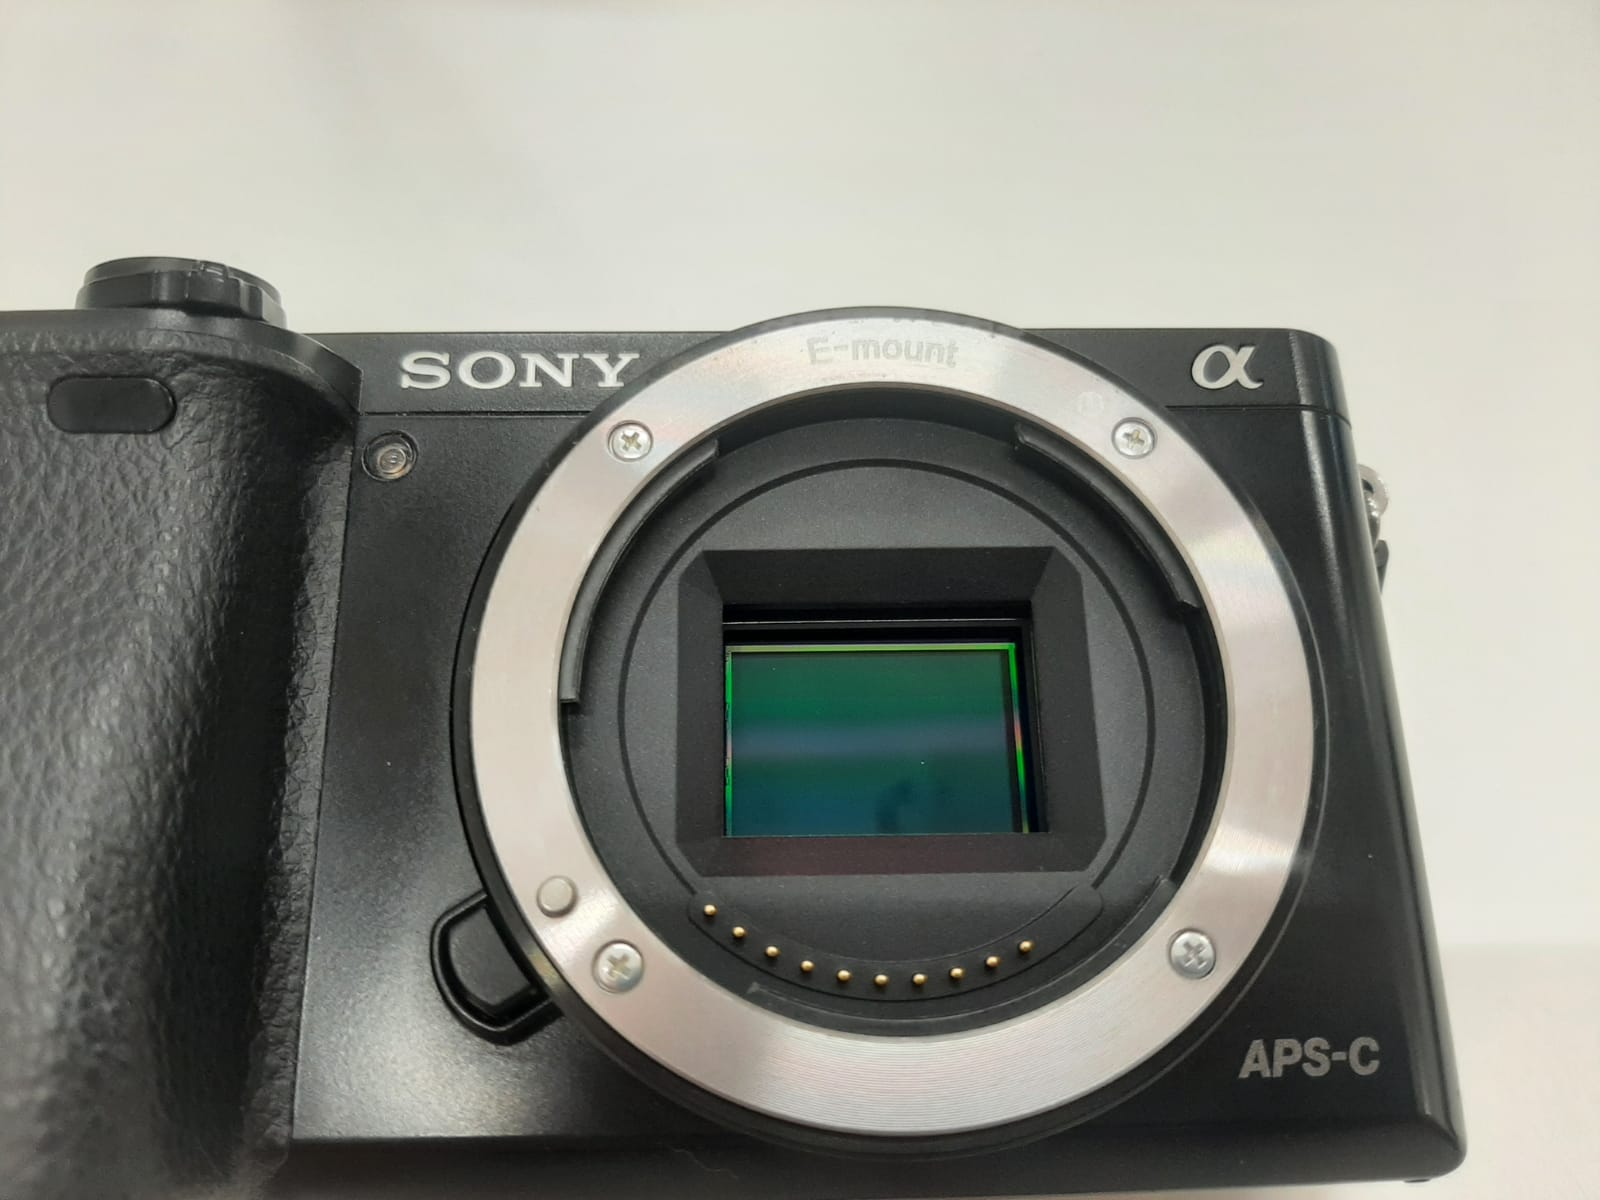
\includegraphics[width=0.7\textwidth]{images/sensor.jpeg}
    \caption{CCD sensor from a SONY Alpha commercial camera.}
    \label{fig:ccdsensor}
\end{figure}
The most commonly used sensor in astronomy is the charge-coupled device (CCD) (\cite{CCDimage}). \autoref{fig:ccdsensor} shows a CCD sensor. On this sensor, the pixels are light-sensitive metal-oxide substrate capacitors, which upon being hit by a photon produce an electric charge which is stored in the capacitor. CCD's are ideal for high-quality scientific cameras because of their high quantum efficiency, i.e. the conversion from impinging photon to electron in the sensor is almost $100\%$. This allows for high quality image generation, even in limited light conditions (\cite{CCDimage}). However, this quality comes at a cost. Firstly, CCD's are faily expensive to produce. This is however not a rarity in space systems. On a more practical level, CCD's suffer from an inherent issue known as "Bloom". This might be familiar to the reader where in overexposed images, or images with very bright areas, the brightness \textit{leaks} into neighbouring pixels. This is a result of overflow in the capacitor bins due to overaccumulation of charge. It might lead to very detrimental results when the exposure is bad. On the other hand, this is contrasted by the possibility to reduce the noise from a variety of sources by a lot as described by \cite{CCDsignal}.\\

After exposure to the image, the CCD is read out sequentially by transferring the charge to an amplification circuit to obtain a voltage. This voltage is then measured, the value digitized as \textit{data numbers} or $DN$ and this result stored in memory (\cite{CCDBook}). In practice, this requires selecting an amount of memory to allocate per pixel, the bit-depth (more memory allows a higher resolution in brightness), and storing the subsequent square array. Common values for bit-depth are 8-bit (allowing 256 different values) and 16-bit (allowing 65536 different values).\\

\begin{figure}[htbp]
    \centering
    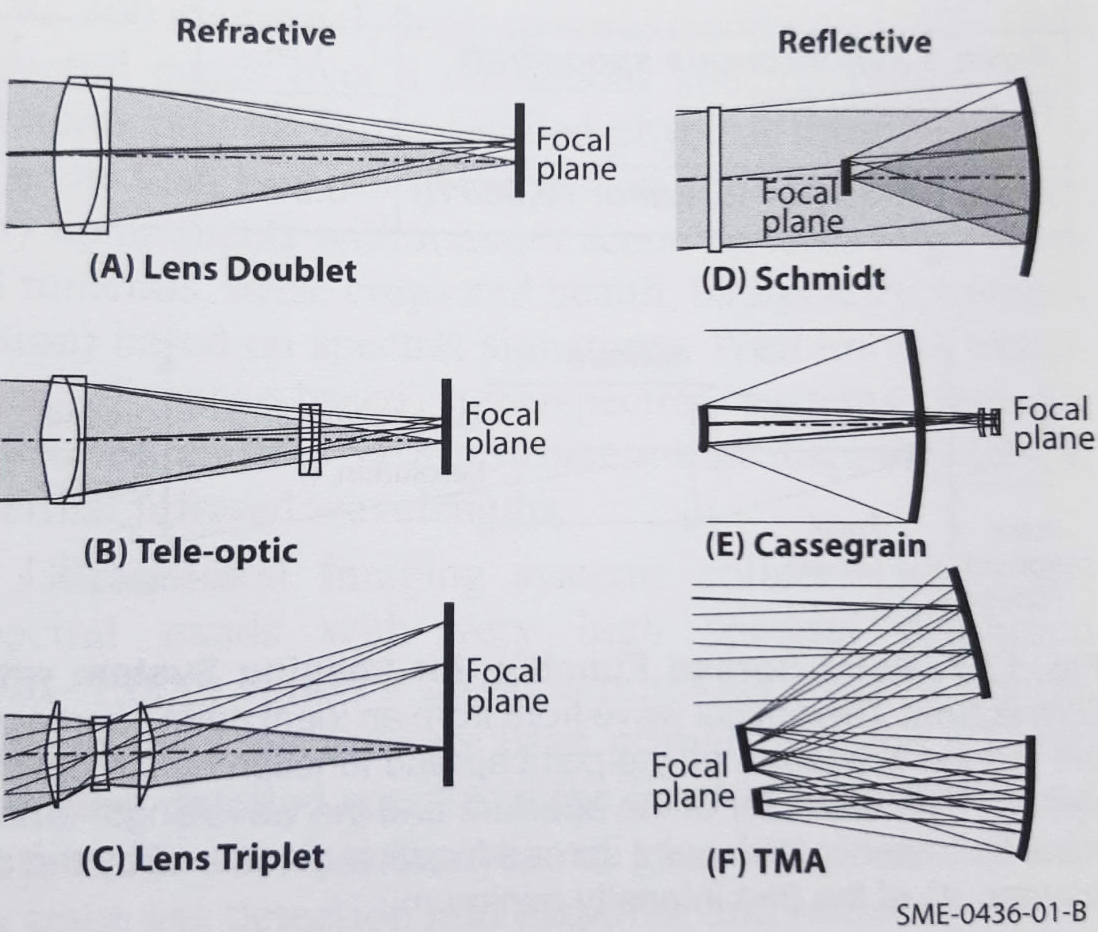
\includegraphics[width=0.5\textwidth]{images/mirrorlens.png}
    \caption{Overview of common mirror and lens setups. (\cite{SMAD})}
    \label{fig:mirrorslenses}
\end{figure}

Optical systems like the CCD commonly require a device to focus incoming light rays onto the focal plane of the sensor. In addition, this allows for capturing photons from a larger area than the area of the sensor itself, therefore increasing the amount of photons coming in, and increasing the image quality. The most common devices are mirrors or lenses. An overview of common arrangements is shown in \autoref{fig:mirrorslenses}. Most of these systems suffer from some abberations, such as, but not limited to:
\begin{itemize}
    \item Chromatic abberation: Different wavelengths of light refract at different angles. Therefore, there is a "prism"-like effect in lens telescopes.
    \item Spherical abberation: Imperfect mirror shapes cause blurring near the edge of the field.
    \item Field curvature: Because of the differing distances light has to travel, a flat object can not be brought to focus exactly on a flat detector.
    \item Coma: Nonuniformity in magnification leads to points near the edge of the field becoming "drawn out".
\end{itemize}
Although good to keep in mind, these abberations can all be corrected for using properly and precisely designed optics. Therefore, luckily the mathematical treatment of these is practically consistent, so more detail on these setups is not required (\cite{SMAD}). In \autoref{sec:opticalnoise}, an overview will be given of problems that are more troublesome to correct for.

\section{Mathematics of Optics}
\label{sec:opticsfundamentals}

After discussing the hardware, in this section a mathematical treatment of the optical systems will be presented. These definitions are needed to accurately assess the images in research. The problem is described by \cite{OpNav} as follows:\\

\textit{"Given the position and velocity of the spacecraft and the target, the camera attitude, and the camera’s optical properties, where should the image of the target appear within a picture?"} \\

\subsection{Target vector}
\cite{OpNav} begins his analysis of the problem by determination of the inertial direction to the target. Because the speed of light is finite, the target will appear on the spacecraft's sensors based on the \textit{apparent position} rather than the actual, geometric position. In an inertial reference frame centered on the barycenter of the solar system:
\begin{itemize}
    \item Calculate the position $\vec{R_{C}}(t)$ and velocity $\dot{\vec{R_{C}}}(t)$ of the camera at time $t$.
    \item Similarly, compute the position $\vec{R_T}(t)$ and velocity $\dot{\vec{R_T}}(t)$ of the target.
    \item The actual (or geometric) relative position $\vec{G}(t) = \vec{R_T}(t) - \vec{R_C}(t)$. Note that this is not the observed position, due to the fact that the target will have moved before the light reaches the camera.
    \item We can iteratively (because of the magnitude of $c$ the required accuracy here is not very high, so some quick iterations suffice) calculate the time $\tau$ which the light takes to reach the sensor from:
\end{itemize}
\begin{equation}
    \tau=|\vec{R_C}(t) - \vec{R_T}(T-\tau)|/c
\end{equation}
\begin{itemize}
    \item The true position corrected for light time becomes: $\vec{T} = \vec{R_C}(T) - \vec{R_T}(t-\tau)$.
    \item Lastly, the effect of \textit{stellar abberation}, which shifts this direction based on the direction of motion of the spacecraft, has to be taken into account. By performing a vector addition from simple geometry, the following equation for the apparent position $\vec{A}(T)$ is obtained:
\end{itemize}
\begin{equation}
    \vec{A}(t) = \vec{T}(t) + |\vec{T}(t)|[\dot{\vec{R_C}}(t)/c]
    \label{eq:apparentposition}
\end{equation}
\autoref{eq:apparentposition} is a formulation of the apparent position of the target as seen from the spacecraft in Newtonian physics. For the proposed research, this is assumed sufficient.

\subsection{Camera Attitude}
With the apparent position vector to the target determined, \cite{OpNav} continues by defining the attitude of the camera.\\

\begin{figure}[htbp]
    \centering
    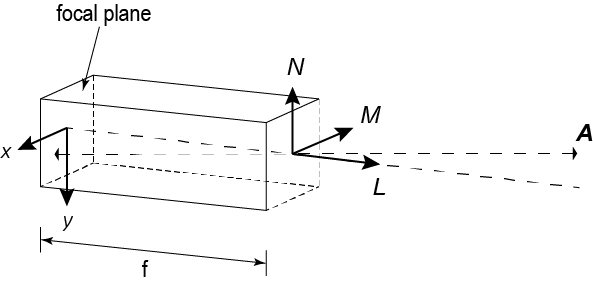
\includegraphics[width=0.6\textwidth]{images/cameracoordinates.png}
    \caption{Illustration of coordinate frames used in the camera attitude determination}
    \label{fig:cameracoordinates}
\end{figure}

Start by determining a cartersian right-handed coordinate system C, using axes M-N-L with the L-axis oriented along the optical axis of the camera, and M and N being arbitrary perpendicular vectors (by convention M+ points to the left and N+ points up, as seen from the focal plane.) \autoref{fig:cameracoordinates} provides a graphical overview of the coordinate system. The transformation from the of the apparent position in the inertial frame $\vec{A^I}$ to the apparent position vector in the camera frame $\vec{A^C}$ is then given by a transformation matric $\mathbf{C}$:
\begin{equation}
    \vec{A^C} = \mathbf{C}\vec{A^I}
\end{equation}
The analysis thus continues to obtain matrix $\mathbf{C}$. Note that merely finding the direction of the L-axis is not sufficient; the camera is capable of rotation along this axis, which will alter the resulting matrix. Matrix $\mathbf{C}$ can be obtained from a sequence of rotations by Euler angles, such as:
\begin{equation}
    \mathbf{C} = \mathbf{R_3}(\phi)\mathbf{R_1}(90^\circ - \delta)\mathbf{R_3}(\alpha + 90^\circ)
\end{equation}
Or alternatively:
\begin{equation}
    \mathbf{C} = \mathbf{R_3}(\phi + 90^\circ)\mathbf{R_2}(90^\circ - \delta)\mathbf{R_3}(\alpha)
\end{equation}
With the standard rotation matrices:
\begin{align}
    \mathbf{R_1}(\theta) &= \begin{bmatrix} 1 & 0 & 0 \\ 0 & \cos{\theta} & -\sin{\theta} \\ 0 & \sin{\theta} & \cos{\theta} \end{bmatrix} \\
    \mathbf{R_2}(\theta) &= \begin{bmatrix} \cos{\theta} & 0 & \sin{\theta} \\ 0 & 1 & 0 \\ -\sin{\theta} & 0 & \cos{\theta}\end{bmatrix} \\
    \mathbf{R_3}(\theta) &= \begin{bmatrix} \cos{\theta} & -\sin{\theta} & 0 \\ \sin{\theta} & \cos{\theta} & 0 \\ 0 & 0 & 1 \end{bmatrix}
\end{align}
Here, $\alpha$ represents the right ascension of the optical axis L and $\delta$ represents the declination. $\phi$ is a thirs twist angle to define the rotation of the camera along the L-axis. For simplicity, it will be assumed that camera attitude is sufficiently known and controllable that this definition of $\mathbf{C}$ holds.\\

\subsection{Projection}
By idealizing the camera's lens to a point, \cite{OpNav} calculates the image's projection as follows. Because of this idealized assumption, Light rays from the target will pass through the point opening in the camera, at the position of the lens (the origin of $\mathbf{C}$). As no lens is present but only a infinitely small hole, the light rays will continue in a straight line until reaching the detector in the focal plane, situated at focal length $f$ behind the camera opening. From simple geometry, \autoref{fig:cameracoordinates} allows finding the so-called \textit{gnomonic} projection in the coordinates of the detector (note that the L-axis, or optical axis is the third axis in the coordinate system):
\begin{equation}
    \begin{pmatrix} x \\ y \end{pmatrix} = \frac{f}{A^C_3}\begin{pmatrix}A^C_1 \\ A^C_2\end{pmatrix}
    \label{eq:cameraprojection}
\end{equation}
The coordinate system shown in \autoref{fig:cameracoordinates} is "upside down", as the camera will project the vector in an inverted position. Note that because the right-hand side of \autoref{eq:cameraprojection} involves a ratio of the components of the apparent position vector, the actual magnitude of this vector is irrelevant, which is confirmed intuitively when considering how a camera normally operates.

\subsection{Lenses and Magnification}
\begin{figure}
    \centering
    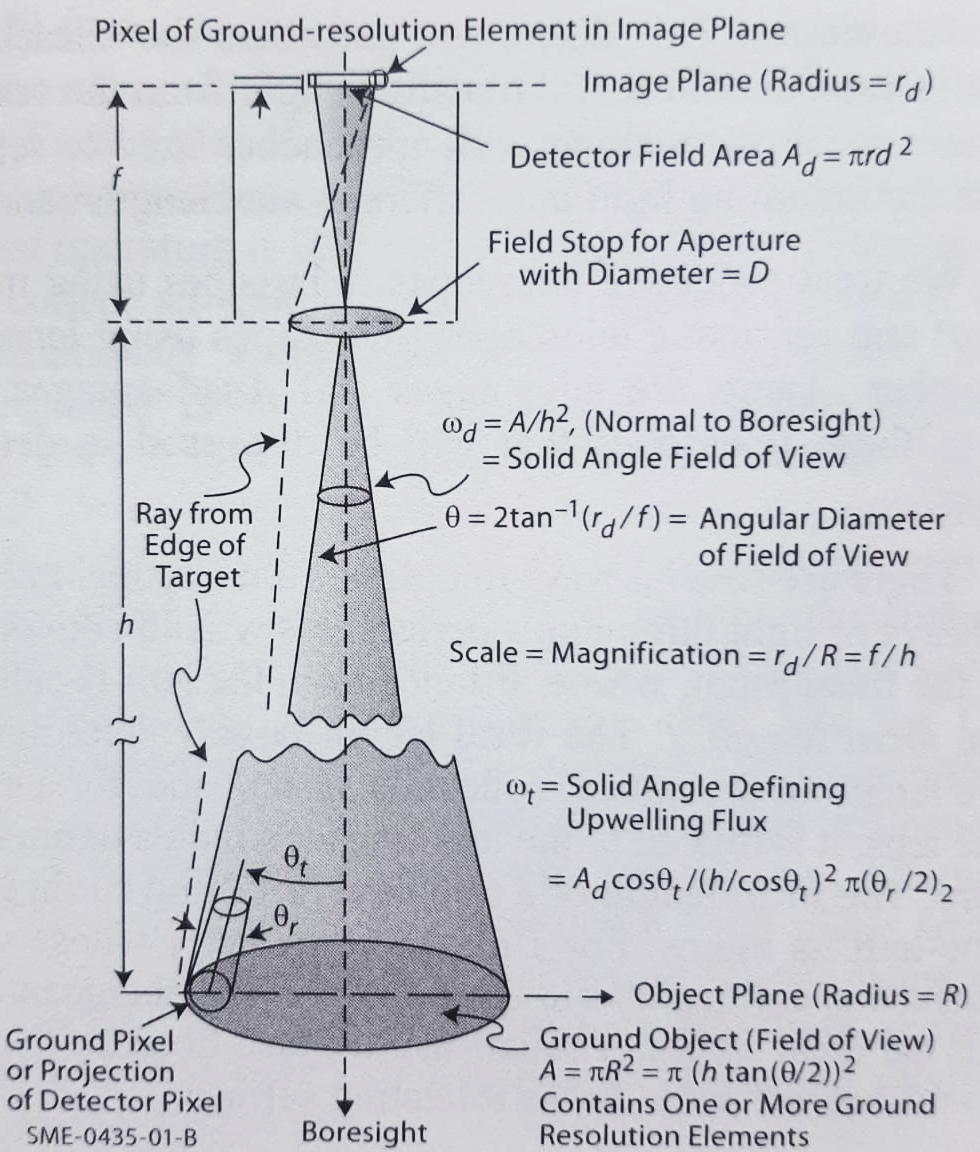
\includegraphics[width=0.6\textwidth]{images/optics.png}
    \caption{Description of elements of an optical system. The presented figure is for a refractive system, although mathematically a reflective system functions similarly. (\cite{SMAD})}
    \label{fig:smadoptics}
\end{figure}
In reality, the lens of a camera is not an infinitely small opening in the front of the camera. For this purpose, lenses, mirrors or a combination of these are used to focus the light onto the sensor as described in \autoref{sec:opticalhardware}. As the advantages and disadvantages of each have already been described there, the explanation presented here will only focus on lenses, although the mathematics are consistent with mirrors with some trivial adjustment which can be derived from geometry. A perfect lens is a device that will focus incoming parallel light rays into a "focal point", where all the rays will exactly converge. This focal point is located at focal length $f$ behind the lens. According to \cite{SMAD}, the requirement of focal length is, in design, often dependent on the actual size of the detector and of the required angular resolution or field of view. Let $M$ be the magnification of the target, defined as the ratio of image dimensions to object dimensions:
\begin{equation}
    M \coloneq \frac{r_d}{R}
\end{equation}
With $R$ the radius of the target and $r_d$ the radius of the detector. It then follows, that for a perfect lens (see \autoref{fig:smadoptics}):
\begin{equation}
    M = \frac{f}{h} = \frac{r_d}{R}
\end{equation}
With focal length $f$ and distance to target $h$ (\cite{SMAD}). Next to the focal length, a second important property of a lens is how much light it collects. The amount of light is a direct function of the collector area. This is often described as the \textit{infinity F-number} or \textit{F-stop}. It is defined as the ratio of focal length to effective aperture of the main lens or mirror:
\begin{equation}
    F\# = \frac{f}{D}
\end{equation}
Assuming a constant photon flux, the number of incoming photons is directly proportional to area. Therefore, image brightness $\propto F\#^{-2}$, making this another property to consider. In practice, the lowest value of $F\#$ used is $0.5$ (\cite{SMAD}).
\subsection{From Projection to Pixel Values}
Rounding out the description of optics, \cite{OpNav} considers the process of converting from the previously found $(x, y)^T$ vector to the measured values in the pixels of the detector. transforming the vector into line $l$ and sample $s$ is done through a linear transformation:
\begin{equation}
    \begin{pmatrix}s \\ l\end{pmatrix} = \begin{bmatrix}K_x & K_{xy} \\ K_{yx} & K_y\end{bmatrix} \begin{pmatrix}x \\ y \end{pmatrix} + \begin{pmatrix} s_0 \\ l_0 \end{pmatrix}
\end{equation}
It will be assumed in further analysis that the used detector has perfectly square pixels. In this case $K_x = K_y$ equalling the side length of a pixel. and $K_{xy} = K_{yx} = 0$. The offset $(s_0, l_0)^T$ corresponds to the offset between the center of the optical axis, where the detector reference frame is located and the origin of the pixel reference frame.\\

With the reference frame defined, the last steps for determining the digital values are defining the incoming light and converting this to pixel values. Firstly, \cite{OpNav} gives for the signal $S(s, l)$ in a pixel measured in electrons:
\begin{equation}
    S(x,l) = A\iiint I(\alpha, \delta, \nu, t)F(\nu)Q(\nu)d\nu d\Omega dt
    \label{eq:pixelsignal}
\end{equation}
With:
\begin{itemize}
    \item Camera aperture $A$
    \item Solid view angle $\Omega$ subtended by a pixel.
    \item Incoming light $I$ as a function of direction $\alpha, \delta$, frequency $\nu$ and time $t$ in units of m$^{-2}$sr$^{-1}$Hz$^{-1}$s$^{-1}$.
    \item A filter on the camera may cause another frequency dependent effect $F(\nu)$.
    \item Because of the usage of the photo-electric effect, there is a \textit{quantum efficiency} $Q(\nu)$, the fraction of generated electrons to incident photons, which is also frequency dependent.
\end{itemize}
The conversion to data numbers is then straightforward from two properties of the conversion process:
\begin{equation}
    DN(s, l) = S(s, l)/g + b
\end{equation}
with $g$ being the gain expressed as $DN$ per electron, and $b$ a constant offset term. These values can then be stored by the detector in a numerical array and used for further processing.
\section{Diffraction Limitation}
\label{sec:opticslimitations}
Of relevance to the research is the most extremely angular resolution achievable by the camera. This is important because of the intent to capture images of far away targets of small size. If all optical abberations are corrected for, which is possible using advanced optics (\cite{SMAD}), and in addition, sufficient noise is removed, which is possibly through a process known as \textit{flat-fielding} (\cite{OpNav}), the limitation to angular resolution is primarily the \textit{Abbe diffraction limit} (\cite{diffractionlimit}). The extent of this limitation is determined by the wavelength of the incoming photons and the aperture of the camera. \autoref{fig:airydiffraction} shows a well known example created by shining a laser beam on a tiny puncture in a screen; effectively creating a minuscule aperture. The diffraction of the light will make discerning further detail in the source of the light impossible. With distance to target $h$, aperture diameter $D$, wavelength $\lambda$ and target resolution limit $X'$, the corresponding relation is:

\begin{equation}
    X' = \frac{h \lambda}{D}
    \label{eq:difflimit}
\end{equation}

\autoref{eq:difflimit} can be used to quickly determine the maximum resolution achievable under the diffraction limit. For high-quality optics in space (i.e. no atmospheric disturbance), this is a fair assumption (\cite{SMAD}). In \autoref{tab:difflimit}, some examples are given for the diffraction limit for visible light of $0.5\mu m$. Even for large apertures\footnote{For reference: the aperture of the Hubble Space Telescope is 2.4m}, it can be seen that the resolution will almost always be larger than the intended target size, with the exception of very close-by targets.\\
\begin{figure}[htbp]
    \centering
    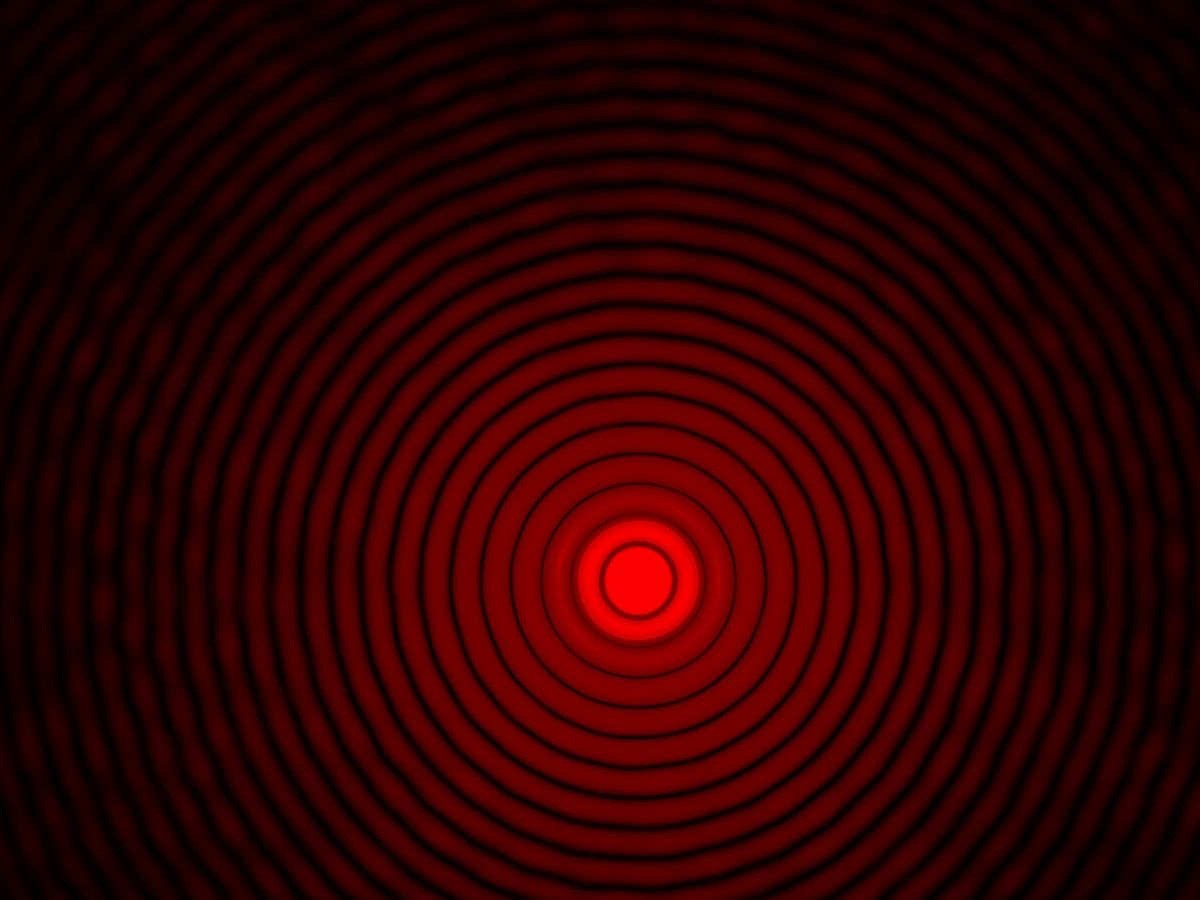
\includegraphics[width=0.6\textwidth]{images/diffraction.jpg}
    \caption{An Airy diffraction disk created by shining a laser on a 90-micrometer hole.}
    \label{fig:airydiffraction}
\end{figure}

\begin{table}[htbp]
\centering
\caption{Examples of diffraction target resolution limit for several aperatures and distances for $\lambda=0.5\mu m$ visible light.}
\label{tab:difflimit}
\begin{tabular}{l|lll}
\textbf{Distance to target} & \textbf{D=0.1m} & \textbf{D=0.5m} & \textbf{D=1m} \\ \hline
10.000 km                   & 50 m            & 10 m            & 5 m           \\
1 Mm                        & 5 km            & 1 km            & 500 m         \\
1 AU                        & 750 km          & 150 km          & 75 km        
\end{tabular}
\end{table}

As the population of NEA's above the lower limit for target size (30 m) is approximately $0.8\cdot10^6$, which can be seen in \autoref{fig:asteroiddetect}, a calculation is possible to judge this distance. Assuming all NEA's are spaced out evenly along Earth's orbit (the best-case scenario), the average distance between two asteroids:
\begin{equation}
    \frac{1.5\cdot 10^8 * 2 \pi}{0.8 \cdot 10^6} = 1178 \mathrm{km}
\end{equation}
From this follows that, on average, only roughly 15 50m asteroids will be resolved by the camera of a spacecraft with a 0.1m aperture. Although overly simplified, it is clear that the asteroids should be taken as a point light source in the camera. As will be explained in \autoref{ch:imageprocessing}, it is often necessary to obtain more than one pixel of information to carry out detailed processing of the image. Luckily, diffraction offers an important solution in the form of the \textit{Point Spread Function} (PSF). As described by \cite{airyfunction}, the idealized PSF of intensity $I$ as a function of dimensionless distance from the optical axis $u$ is given by the airy disk, shown in \autoref{fig:airydiffraction}:
\begin{equation}
    I(u) = \left(\frac{2J_1(u)}{u}\right)^2
\end{equation}
With:
\begin{equation}
    u = \frac{\pi}{\lambda}D\theta
\end{equation}
And $J_1$ the first Bessel function of the first kind. The presented function is a simplification assuming no obstruction of the aperture (such as would occur in a reflector telescope). These functions are easily generated by e.g. Python, and an example of the result in dimensionless $u$ quantities is shown in \autoref{fig:airyfunction}. This function can used to model the distribution of incoming light from a target asteroid.

\begin{figure}[htbp]
    \centering
    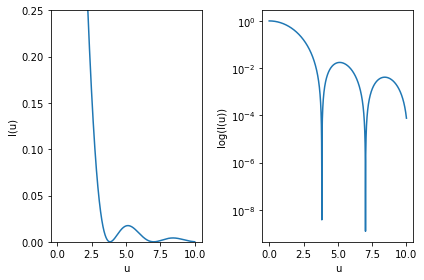
\includegraphics[width=0.6\textwidth]{images/airyfunction.png}
    \caption{Simulated intensity of airy disk in 2D in dimensionless units $u$}
    \label{fig:airyfunction}
\end{figure}

\section{Noise and Bias}
\label{sec:opticalnoise}
In modeling the optical system, there are several factors that need to be considered with regard to the signal to noise ratio of the produced data. There are several sources of noise that can not be compensated for completely, and thus need to be taken into account. In order of decreasing influence, they are (\cite{OpNav}; \cite{SMAD}):
\begin{enumerate}
    \item Dark Current $N_d$: thermal effects will spontaneously produce electrons in the detector, even in the absence of light. These electrons are indistinguishable from "real" electrons generated by incident light, and therefore deteriorate the signal. Dark current is mainly a function of temperature, increasing with a warmer sensor.
    \item Read Noise $N_r$: As with any system, interaction will alter the state of the system. Therefore, reading out the amount of charge in the detector will have an influence on the detector, and this is mainly a property of the quality of the detector electronics.
    \item Fixed Pattern Noise $N_f$: A fixed pattern of dark current, always causing a certain offset in the data. This can have quite a large effect on the image quality, but as the pattern is constant (only being affected slowly by e.g. radiation damaging the sensor), it can be compensated for by calibration.
    \item Shot noise $N_s$: The photon flux is not a continuous process, but rather a poisson process. Therefore, it has an additional random component in when photons reach the detector. This noise decreases with higher numbers of photons (i.e. brighter targets or longer exposure).
    \item Quantization noise $N_q$: Because the analog voltage of the detector gets converted to a digital signal, a certain amount of noise is introduced. 
\end{enumerate}
The total noise can be determined as:
\begin{equation}
    N^2 = N_d^2 + N_r^2 + N_f^2 + N_s^2 + N_q^2
    \label{eq:noisecombined}
\end{equation}

In addition, the background light level should be taken into account as an additional noise source. \cite{nightsky} gives an estimate of $B_e = 3\cdot 10^{12}$ photons sr$^{-1}$ s$^{-1}$ m$^{-2}$ in the absence of large bodies nearby (e.g. the Moon). \cite{thesisspacebased} suggests taking the influence of starlight into account. Stars are roughly constant throughout the night sky, with the exception of the galactic plane. \cite{starlight} estimate a mean flux from starlight of between $B_e = 2\cdot 10^{12}$ and $ 3\cdot 10^{12}$ photons sr$^{-1}$ s$^{-1}$ m$^{-2}$ at angular distances over $30^\circ$ from the galactic plane. When approaching the galactic plane, the intensity increases up to $6 \cdot 10^{12}$ to $8 \cdot 10^{12}$ photons sr$^{-1}$ s$^{-1}$ m$^{-2}$ at the galactic plane. 

According to \cite{thesisspacebased}, the sources large enough to consider for the application are the dark current and read noise, as well as the background light. This brings a final estimate of the Signal-to-noise ratio by dividing the signal by the Root-Sum-Square of the noise sources(\cite{OpNav}):
\begin{equation}
    SNR = \frac{S_{target}}{\sqrt{N_d^2 + N_r^2 + B_e^2}}
\end{equation}
In practice, SNR's of above three can be used, whereas lower SNR's might yield problems for the detection (\cite{SMAD}). Some examples of typical values from \cite{NASAreport} can be seen in \autoref{tab:typicalcamera}.

\begin{table}[htbp]
\centering
\caption{Typical values for spacecraft optical system}
\label{tab:typicalcamera}
\begin{tabular}{ll}
\textbf{Parameter}               & \textbf{Typical value} \\ \hline
Aperture {[}m{]}                 & 0.5                    \\
FOV {[}deg{]}                    & 10.6 x 5.3             \\
Number of pixels {[}V x H{]}     & 9232 x 9216            \\
Exposure time {[}s{]}            & 24                     \\
Dark current {[}e-/h{]} at 100 C & 2                      \\
Readout noise {[}e-{]}           & 4                      \\
Quantum efficiency {[}\%{]}      & 88                    
\end{tabular}
\end{table}